\documentclass[10pt,a4paper]{article}
\usepackage[margin=2.2cm]{geometry}
\usepackage{amsmath,amssymb,graphicx,booktabs,caption,float,xcolor,enumitem}
\usepackage[colorlinks=true,linkcolor=blue!50!black,urlcolor=blue!50!black]{hyperref}
\captionsetup{font=small,labelfont=bf}
\setlist{itemsep=1pt,topsep=3pt}
\graphicspath{{figures/}}
\newtheorem{result}{Result}

\title{\textbf{A finite fact-flow model}\\[2pt]
\textbf{Finite size explains the size of the controller's effect}}
\author{Claude (theory work, \nolinkurl{analysis/theory_claude/phenomenological_fact_flow/})}
\date{28 October 2026}

\begin{document}
\maketitle

\begin{abstract}
\noindent
The mean-field fact-flow model of 27 October reproduces both phenomena qualitatively, but its controller effect is 3--10
times smaller than the simulator's. Here the same model is made finite: individual agents, individual facts, and a board
of whole posts, so a fact can die out. The parameters are those of the mean-field model, chosen before any run; nothing
is fitted. All six predictions written in advance are met:
\begin{itemize}
\item most of the agents' own facts die out at short memory (``diversity collapse''), as in the simulator;
\item the controller's effect becomes 4 times larger and close to the simulator's;
\item the reading reversal remains, with its crossover at $\rho\approx0.5$--$0.6$;
\item removing the controller's facts leaves lasting damage;
\item persistence is slow;
\item copying the swarm with fixed facts drives the effect to the mean field, almost number for number as in the
  simulator.
\end{itemize}
A controlled comparison attributes about half of the finite-size amplification to the controller's evidence being
concentrated in few facts, which survive, while the agents' spread-out evidence collapses. The reading increment $D$ is
2--3 times too small, and the $K$-projects scaling is not reproduced.
\end{abstract}

\section{The finite model}
Same rules as the mean-field model (report of 27 October, Eqs.~1--5), but stochastic and finite. All choices were
logged before running.
\begin{itemize}
\item $N=24$ agents. Each holds a set of facts out of $F_A=16$ agent facts and $F_C=4$ controller facts. Each starts with
  one agent fact (8 facts held twice).
\item A board of posts. Agents read from the $W=48$ newest posts that are not their own.
\item Time step $dt=0.05$. Each agent acts with probability $dt$, and each held fact is forgotten with probability
  $1-\rho^{dt}$.
\item \textbf{An action:}
  \begin{enumerate}
  \item read $q$ posts and remember their facts;
  \item vote for the wrong answer $A2$ with probability
    \begin{equation}\Phi_2=\sigma\big(h_0+\beta_C\,c-\beta_A\,a\big),\label{eq:vote}\end{equation}
    where $a$ and $c$ are the numbers of agent and controller facts the agent holds;
  \item post one fact: an agent fact with weight $\kappa_A a$, a controller fact with weight $\kappa_C c$, or a
    background post with weight $\kappa_0$. Reposting is neutral ($\varepsilon=1$), as in the best mean-field version.
  \end{enumerate}
\item \textbf{The controller} posts a random controller fact at rate $\lambda_0=1$ until $T=30$.
\item \textbf{Observables} as before, as differences between a controlled and a silent run with the same random seed, 400
  pairs per point.
\end{itemize}
Parameters: $\beta_A=\beta_C=0.5$, $h_0=\ln\tfrac12$, $\kappa_A=\kappa_C=1$, $\kappa_0=0.2$. No Bayesian engine and no
task world are used.

\section{Results}
\subsection{Diversity collapse}
\begin{figure}[h]
\centering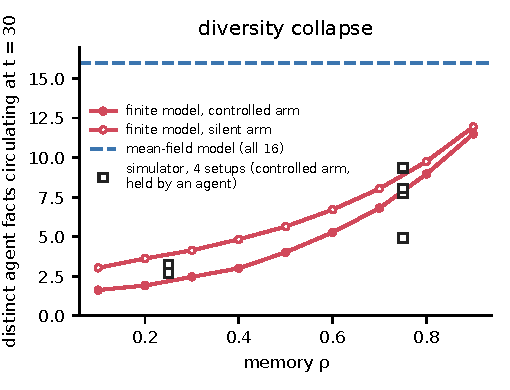
\includegraphics[width=0.52\linewidth]{fig2_diversity.pdf}
\caption{\textbf{Diversity collapse.} Distinct agent facts still circulating at $t=30$, held or on the board. The mean
field keeps all 16. In the finite model most die out at short memory, and the controlled arm loses more. Simulator points:
distinct agent facts held by at least one agent, controlled arm, in all four setups.}
\label{fig:div}
\end{figure}
\begin{result}[F1, met]
At $\rho=0.1$ only 1.6 of the 16 agent facts are still circulating at $t=30$ in the controlled arm, 2.5 at $\rho=0.3$,
6.8 at $\rho=0.7$ and 11.5 at $\rho=0.9$ (Fig.~\ref{fig:div}). All 4 controller facts survive. The simulator shows the
same collapse: about 3 agent facts at $\rho=0.25$ and 5--9 at $\rho=0.75$.
\end{result}

\subsection{The controller effect and the reversal}
\begin{figure}[h]
\centering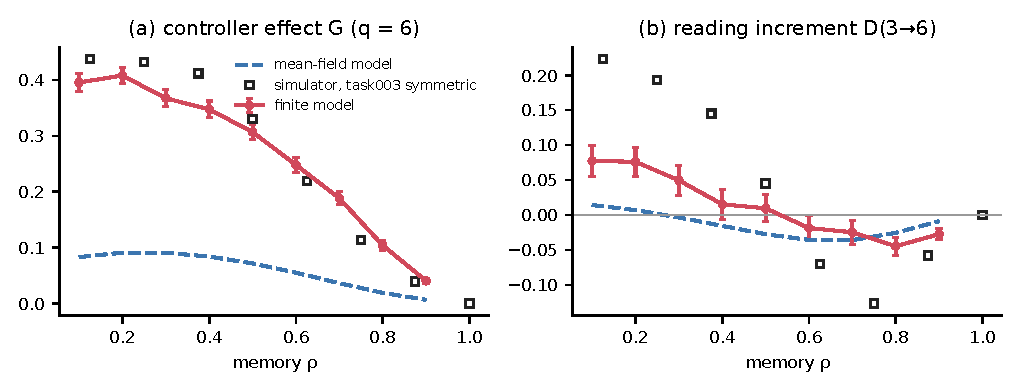
\includegraphics[width=\linewidth]{fig1_reversal.pdf}
\caption{\textbf{Finite against mean-field model}, with the simulator's task003 symmetric setup for reference (not
fitted). (a) The finite model's controller effect is about 4 times the mean field's and close to the simulator's. (b) The
reversal remains; its crossover moves to $\rho\approx0.5$--$0.6$, as in the simulator, but its size is 2--3 times
smaller than the simulator's.}
\label{fig:rev}
\end{figure}
\begin{result}[F2, F3, met]
$G(q=6)$ is 0.31--0.41 for $\rho\le0.5$, against 0.07--0.09 in the mean field; the simulator has 0.33--0.44.
$D(3\to6)=+0.078\pm0.011$ at $\rho=0.1$ and $-0.044\pm0.007$ at $\rho=0.8$. The crossover lies between 0.5 and 0.6;
the simulator's task003 symmetric setup crosses between 0.5 and 0.625 (Fig.~\ref{fig:rev}).
\end{result}

\subsection{Persistence}
\begin{figure}[h]
\centering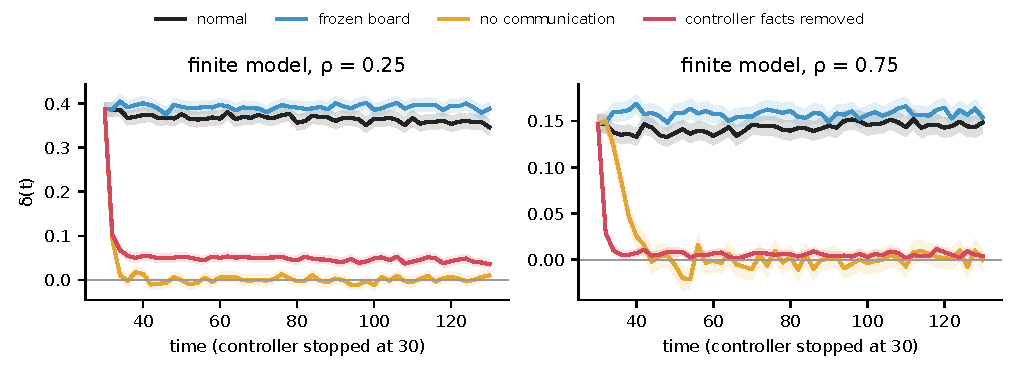
\includegraphics[width=\linewidth]{fig3_persistence.pdf}
\caption{\textbf{The four continuations in the finite model} ($q=6$; 95\% bands).}
\label{fig:pers}
\end{figure}
\begin{result}[F4, F5]
\begin{itemize}
\item \textbf{Removal (F4, met):} after the controller's facts are removed, a residual of $+0.036$ remains at
  $\rho=0.25$ (the simulator's task003 symmetric: $+0.04$). This is lasting damage: agents' facts that died out during
  control do not return.
\item \textbf{Normal continuation (F5):} the effect declines slowly, $0.388\to0.347$ over 100 time units at
  $\rho=0.25$, and stays flat at $\rho=0.75$. There is no fast plateau. This resembles task003's flat persistence.
\item \textbf{The other two continuations} behave as in the simulator: the frozen board keeps the effect, and no
  communication removes it, with a slight transient rise at $\rho=0.75$ (Fig.~\ref{fig:pers}).
\end{itemize}
\end{result}

\subsection{Scaling}
\begin{figure}[h]
\centering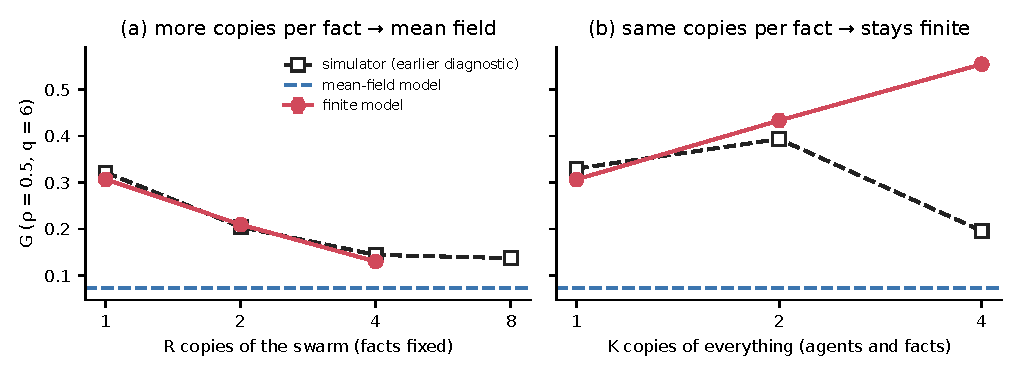
\includegraphics[width=\linewidth]{fig4_scaling.pdf}
\caption{\textbf{Scaling.} (a) Copying the swarm $R$ times with the facts fixed raises the copies per fact, and the
effect falls toward the mean field, nearly as in the simulator's earlier diagnostic. (b) Copying agents and facts
together keeps the copies per fact. The finite model stays far from the mean field, but rises at $K=4$ where the
simulator falls.}
\label{fig:scale}
\end{figure}
\begin{result}[F6, met]
With $R$ copies of the swarm (24$R$ agents, 48$R$ board slots, controller rate $\times R$, same 20 facts), $G$ falls as
0.307, 0.209, 0.130 for $R=1,2,4$, toward the mean-field 0.072. The simulator's earlier diagnostic gave 0.322, 0.204,
0.144. With $K$ copies of everything, $G$ does not approach the mean field (0.43 at $K=2$, 0.56 at $K=4$). The simulator
instead falls at $K=4$ (0.20). In the simulator a single fact is less informative at larger $K$, which the model does not
represent.
\end{result}

\subsection{Why finite size enlarges the effect}
\begin{figure}[h]
\centering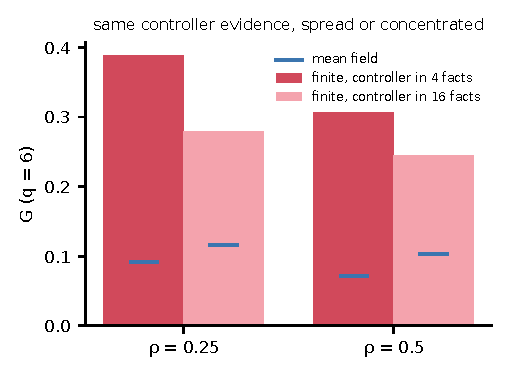
\includegraphics[width=0.52\linewidth]{fig5_concentration.pdf}
\caption{\textbf{Concentration.} The same total controller evidence ($F_C\beta_C=2$), carried by 4 facts or by 16. Bars:
finite model. Marks: mean field at the same parameters. Spreading the controller's evidence over many facts brings the
finite model closer to the mean field.}
\label{fig:conc}
\end{figure}
\begin{result}[asymmetric extinction]
The controller's evidence sits in 4 facts, each kept in many copies, so all 4 survive. The agents' evidence is spread over
16 facts, most of which die out. Extinction therefore removes the swarm's own evidence, which protects it, but not the
controller's. With the same total controller evidence spread over 16 facts (Fig.~\ref{fig:conc}), the finite effect
falls from 0.39 to 0.28 ($\rho=0.25$) and from 0.31 to 0.25 ($\rho=0.5$). Its ratio to the mean field falls from 4.2 to
2.4. So concentration accounts for about half of the finite-size amplification, and the collapse of the agents' own
evidence for the rest.
\end{result}
\emph{Note on procedure.} The first run of this check kept $\beta_C$ fixed while spreading the evidence. That raised the
controller's total evidence and $G$ in both models, so the stated prediction was not met. The equal-evidence run above is
the control that was described before running. Both runs are kept (\nolinkurl{findings/step3_mechanism*.csv}), and the
error is logged.

\section{What this means for the theory}
\begin{itemize}
\item \textbf{The minimal model of both phenomena is a finite one.} Fact flow (memory $\leftrightarrow$ board), a
  threshold vote, and finite numbers of agents, board slots and facts. With parameters set before any run, it gets:
  \begin{itemize}
  \item the size of the controller's effect;
  \item the reversal and its crossover;
  \item the diversity collapse;
  \item the lasting damage after removal;
  \item slow persistence;
  \item the replicated-swarm scaling.
  \end{itemize}
\item \textbf{The effective finite size is the number of copies per fact.} Roughly agents per fact and board slots per
  fact, not the number of agents. More copies per fact means less extinction and an approach to the mean field.
\item \textbf{The key asymmetry is concentration.} The controller recycles a few facts that survive. The swarm's evidence
  is spread over many facts that die out.
\end{itemize}

\paragraph{What is not explained yet.}
\begin{itemize}
\item The reading increment $D$ is 2--3 times smaller than the simulator's.
\item The $K$-projects scaling at $K=4$.
\item The task difference in persistence. Object Placements fades, while this run, at neutral reposting, persists. In
  the finite model, the vote gating $\varepsilon$ and the measured counter-evidence strength $\beta_A$ have not yet been
  varied.
\end{itemize}

\section{Next steps}
\begin{enumerate}
\item \textbf{The four setups in the finite model.} Put each setup's measured strengths $(h_0,\beta_A,\beta_C)$ (report
  of 28 October) into the finite model, nothing else changed. Do the crossovers come out in the simulator's order? Does
  the symmetric/no-proof difference appear in the effect size and in persistence?
\item \textbf{The persistence task difference.} Vary the vote gating $\varepsilon$ in the finite model ($1$ against
  $0.75$, the two values that separated persistent from fading effects in the mean field). Prediction to fix in advance:
  lower $\varepsilon$ gives fading over tens of time units, as in Object Placements.
\item \textbf{An analytic finite-size correction.} Treat the survival of each fact as a branching process, with the
  rates of the mean-field model, to predict the number of surviving facts $F_{\rm eff}(\rho)$. Feed $F_{\rm eff}$ back
  into the mean-field equations. This would turn the finite model's main effect into a formula.
\end{enumerate}

\end{document}
